\section{Cel i zakres pracy}

W pracy dokonano analizy porównawczej trzech wybranych frameworków serwujących dane: Django, .NET oraz NestJS.
Pod uwagę został wzięty aspekt czasu odpowiedzi w różnych warunkach.
Badanie ma na celu wskazać mocne oraz słabe strony każdego z porównywanych narzędzi.
Badany jest wycinek rzeczywistości, który najlepiej jest przedstawiać poprzez analizę porównawczą.
Bezwzględne wartości mogą się różnić w zależności od warunków uruchomienia, natomiast relacje między badanymi obiektami powinny być stale zauważalne.


Testy można podzielić na rodzaje pod różnymi względami. 
Podstawowy podział testów został zaprezentowany na rysunku \ref{rys:test-types}\cite{atlassianRneRodzaje}.
\begin{figure}[!hb]
	\centering 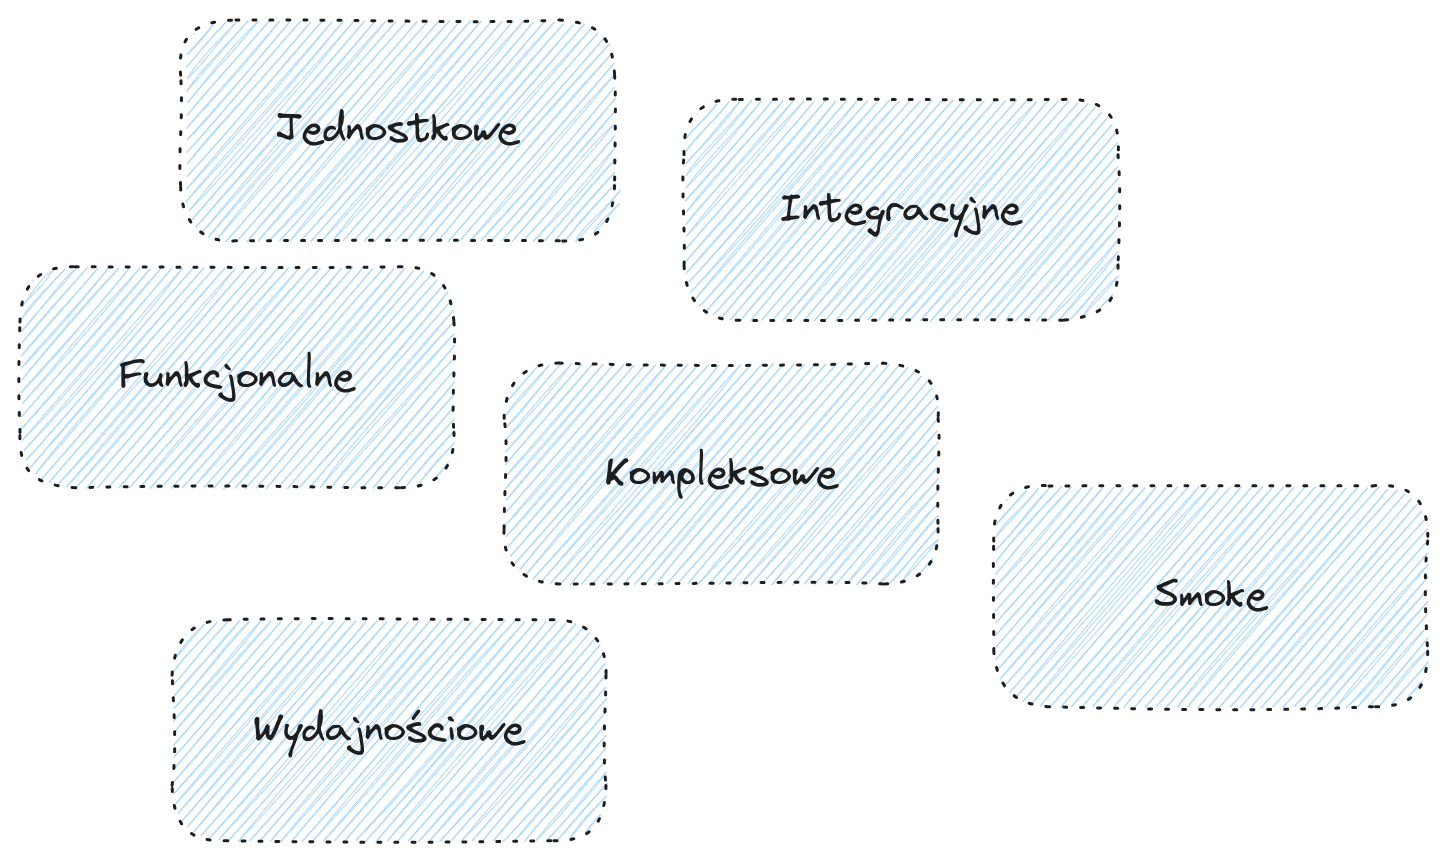
\includegraphics[width=1\linewidth]{rysunki/test-types.png}
	\caption{Rodzaje testów}
	\label{rys:test-types}
\end{figure}
Testy jednostkowe są pisane na stosunkowo niskim poziomie.
Nie jest jednoznacznie zdefiniowane czym jest jednostka która jest testowana.
Czasami jest to jedna funkcja, czasem jeden moduł.
Wszystko zależy od kontekstu badanego rozwiązania.
Różnią się szybkością działania.
Nie jest potrzebna rozbudowana infrastruktura.
Dzięki temu można je uruchamiać często.

Kolejnymi testami, realizowanymi na wyższym poziomie są testy integracyjne.
Służą one badaniu współdziałania różnych modułów ze sobą. 
Do ich uruchomienia potrzebne jest zestawienie kilku modułów ze sobą więc wymagają one zazwyczaj większej infrastruktury niż testy jednostkowe.
Wiąże się to z ograniczeniami związanymi ze zwiększonymi kosztami czasowymi oraz często, powiązanymi z tym, kosztami finansowymi.

Testy funkcjonalne nastawione są na sprawdzenie wymagań biznesowych aplikacji.
Ich złożoność podobna jest do testów integracyjnych.
Dziedziną badania jest sprawdzenie czy kluczowe elementy ich funkcjonalności są realizowane.

Kompleksowe testy służą do badania całej aplikacji.
Testy te wymagają uruchomienia całego systemu w celu jego przetestowania.
Z powodu ich kosztowności zaleca się ograniczenie liczby tych testów do minimum.
Uruchomienie ich najlepiej weryfikuje czy badana aplikacja działa.

Testy akceptacyjne służą do weryfikacji czy kluczowe wymagania biznesowe są realizowane.
Wymagają one również uruchomienia całej aplikacji przez co są kosztowne.

Smoke testy są rodzajem testów, które mają wyłapać błędy widoczne na pierwszy rzut oka.
Polegają na pobieżnym przejściu przez dowolny fragment systemu.
Jest to szybka weryfikacja czy podstawowy element systemu działa jak powinien.

Testy wydajnościowe służą sprawdzeniu czy w wymaganym obciążeniu aplikacja zachowuje się poprawnie.
Pomagają znaleźć wąskie gardła systemu i zapobiec przerwie w działania w przypadku wzrostu obsługiwanych użytkowników lub zwiększenia liczby przetwarzanych danych,

Wraz z wchodzeniem na wyższy poziom testowania koszty testów rosną \cite{testerzyPiramidaTestw}.
Stąd, istnieje piramida testów prezentująca zależność liczby testów w funkcji ich rodzaju.
Piramida ta została zaprezentowana na rysunku \ref{rys:test-pyramid}.
\begin{figure}[!hb]
	\centering 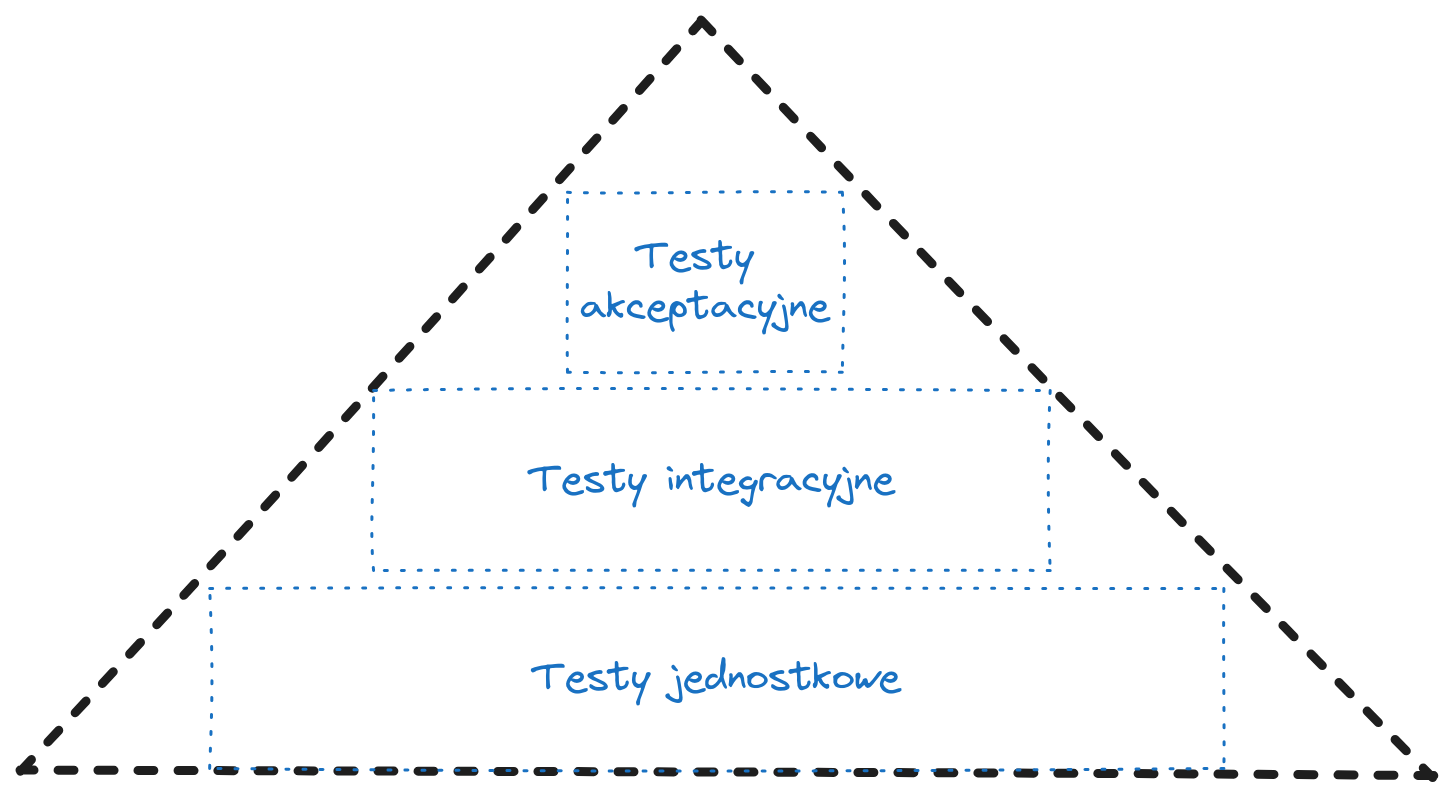
\includegraphics[width=1\linewidth]{rysunki/test-pyramid.png}
	\caption{Piramida testów}
	\label{rys:test-pyramid}
\end{figure}
Testy jednostkowe są realizowane na najniższym poziomie piramidy, a więc tego rodzaju testów powinno być najwięcej jako, że są tanie w utrzymaniu.
Wraz ze wzrostem poziomu piramidy, koszt utrzymania oraz uruchomienia testów rośnie.
Sposób podziału testów jest umowny więc wszystkie nie wymienione rodzaje testów również znajdują się w piramidzie obok najbliższego im rodzaju testów.


Testy przeprowadzone w niniejszej pracy przynależą do kategorii testów wydajnościowych.
Są to kluczowe testy zapewniające o jednym z istotnych aspektów dobrze działającego oprogramowania.
Ich zadaniem jest identyfikacja obszarów ryzyka zachowania w czasie, wykorzystania zasobów oraz przepustowości \cite{testerzyTestowanieWydajnoci}.

\begin{figure}[!hb]
	\centering 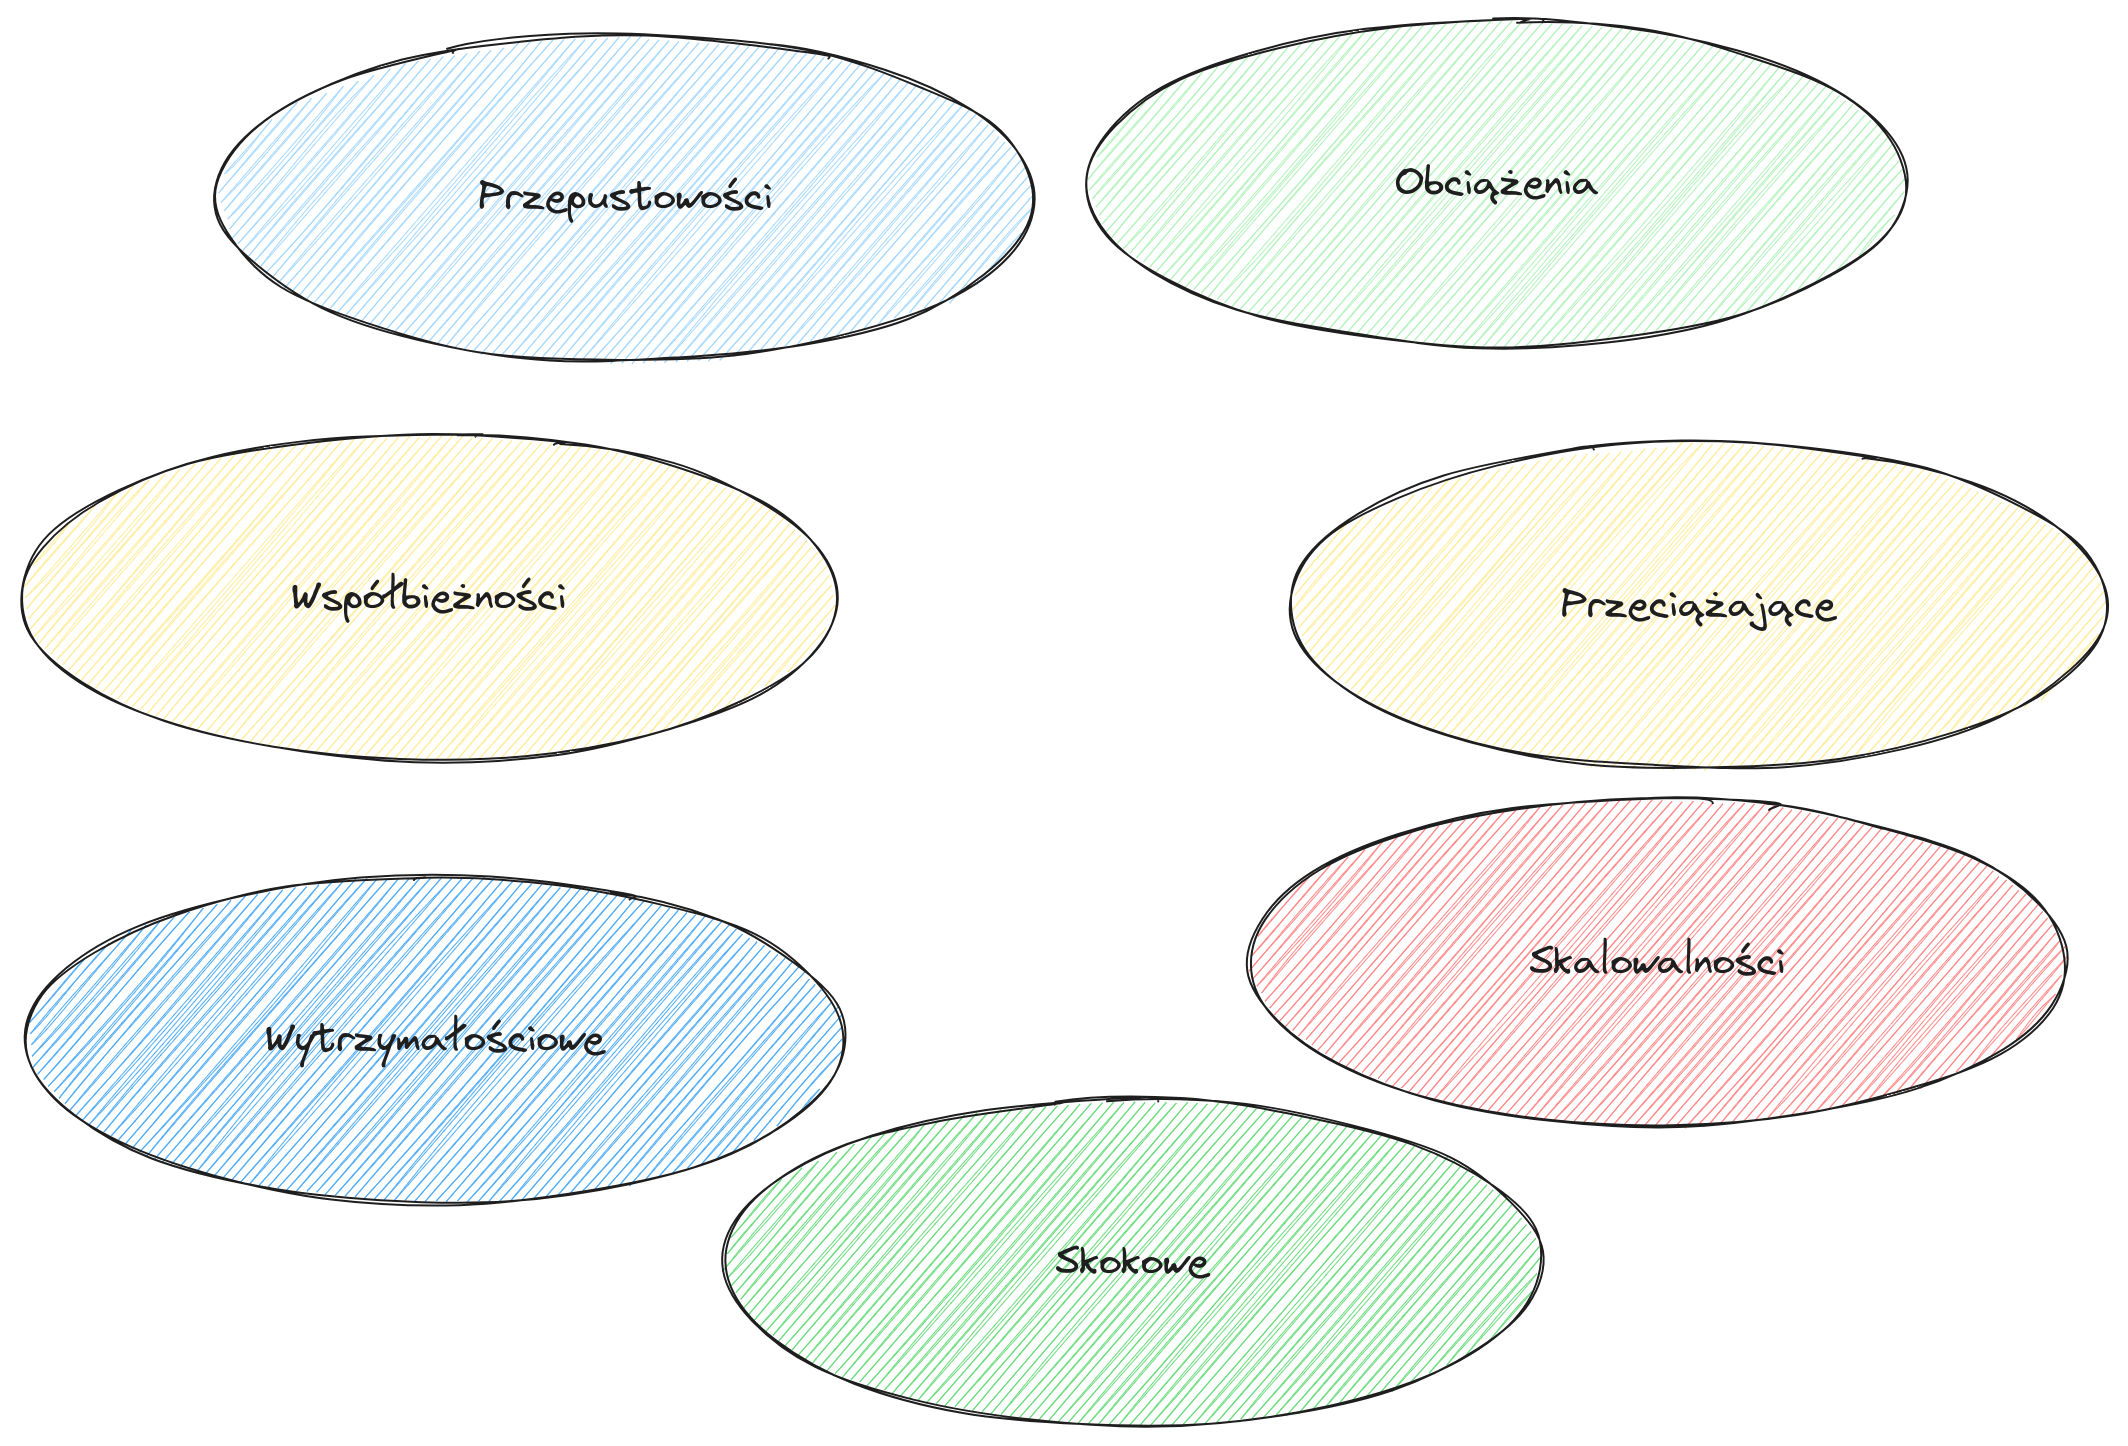
\includegraphics[width=1\linewidth]{rysunki/performance-tests.png}
	\caption{Typy testów wydajnościowych}
	\label{rys:performance-tests}
\end{figure}

Typy testów wydajnościowych zostały zaprezentowane na rysunku \ref{rys:performance-tests}.

Testowanie obciążenia to badanie zdolności systemu do obsługi wzrastającego obciążenia przy realistycznych, przewidywanych liczbach użytkowników mających interakcje z systemem.

Testowanie przeciążające to badanie realizowane przy danych przekraczających realistyczne obciążenie. 
Ma ono na celu znalezienie granicy.

Testowanie skalowalności polega na zbadaniu granic funkcjonowania systemu przy zachowaniu większości pierwotnych założeń.
Pozwala ono na monitorowanie i wczesne reagowanie gdy system wraz z rozwojem stopniowo przekracza bariery wytyczonych wymagań.

Testowanie skokowe to badanie reakcji systemu na nagły, chwilowy wzrost obciążenia.
System powinien być w stanie wrócić no normalnego funkcjonowania, gdy obciążenie wróci do początkowego stanu.

Testowanie wytrzymałościowe skupia się na ocenie działania system w dłuższym okresie specyficznym dla rozwiązania.
Chodzi o drobne uchybienia, które wraz z czasem działania mogą urosnąć do rangi poważnych błędów.
Mogą to być np. błędy obliczeń związane z zaokrąglaniem lub wycieki pamięci.

Testowanie współbieżności służy do sprawdzenia czy system działa poprawnie w przypadku przeprowadzania równoległych operacji.
Jest to zazwyczaj trudny obszar do badania.

Testowanie przepustowości daje ocenę granic działania systemu zgodnie z wymaganiami przy zwiększonej liczbie aktorów mających interakcje z systemem.

Z innego punktu widzenia testy można podzielić na statyczne oraz dynamiczne.
Testowanie statyczne wiąże się ze sprawdzeniem wymagań, architektury rozwiązania w celu znalezienia wąskiego gardła.
Czasami oznacza to również sprawdzenie używanych algorytmów.
Jest to bardzo ważna weryfikacja, ponieważ może zostać zrobiona w początkowej fazie projektu.
Poprawa problemu we wczesnej fazie zazwyczaj sprawia że jest on zdecydowanie mniej kosztowny.
Testowanie dynamiczne to testy jednostkowe, integracyjne, akceptacyjne, które zazwyczaj powstają wraz z rozwojem systemu.
Ich celem jest zwrócenie uwagi na problemy niedostrzeżone w fazie testowania statycznego.
